We looked for users with geographical information available. Information of departments in Argentina (second order division of administration of the country) was collected from the 2010 Census (citation needed). Then, a lookup was made for users with location matching those departaments, balancing the number of users per province.  \textit{tweepy} was used to interact with the Twitter API. 

Although the retrieval of users was attempted on each department, they mainly concentrate around some cities. This phenomenon is due to limitations on the geographical information that Twitter makes available. As our unit of study is the province, this is not an issue.

From these users, their entire tweetlines were retrieved. Tweets were tokenized using \emph{NLTK}\cite{bird2009natural}, which has a special algorithm for this kind of text. Hashtags and mentions to users were removed, and remaining words were downcased, and repeated vowels normalized up to three repetitions (``woaaa'' instead of ``woaaaaaa''). 

As already done with respect to users, the number of words per province was balanced. Table \ref{tab:summary_tweets} lists the figures for the collected dataset.

\begin{table}[b]
\begin{center}

\begin{tabular}{lrrr}
            & Total   & $\mu$   & $\sigma$ \\ % &           STD 
\hline 
Words       &  647M   &  28.14M & 6.64M  \\ %&  3.325680e+06 \\
Tweets      &  80.9M  &  3.51M  & 0.91M  \\ %&  4.571673e+05 \\
Users       &  56.2K  &  2.44K  & 0.04K  \\ %&  1.947665e+01 \\
Vocabulary  &   7.5M  &  0.32M  & 0.04M  \\ %&  2.619165e+04 \\

\end{tabular}


\caption{Dataset summary information. Total figures are provided, along province-level mean and deviation }
\label{tab:summary_tweets}
\end{center}
\end{table}




\begin{figure*}[t]
    \centering
    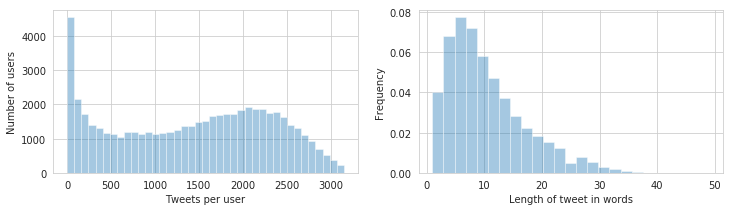
\includegraphics[width=\textwidth]{./images/dataset_histograms.png}
    \caption{Distributional figures of the dataset. First figure shows the distribution of tweets per user. The second figure plots the distribution of the length (in words) of a tweet} 
    \label{fig:tweets_distribution} 
 \end{figure*}



It is well known that Twitter vocabulary tends to be very noisy \cite{kaufmann2010syntactic} with lots of words that come from contractions, non-normal spellings (such as vocalizations), typos, etc. Only words occurring more than 40 times, and being used by more than 25 users are taken into account. This removes about 1\% of the total words and reduces vocabulary from 2.3 million words to around 135 thousand words. 

While this normalization seems insufficient for most analysis, it is acceptable for our study as the phenomenon of locally-used words would emerge in spite of different spellings, typos, and other morphological variations. Indeed, the same word might appear in several different variations or spellings but with one normalized form which would be the more frequent.







